\subsection*{Zadanie 13. (0-6)}
W kartezjańskim układzie współrzędnych kreślimy dwie parabole:
\begin{itemize}
    \item $f(x) = -\frac{1}{4}x^2-2$
    \item $g(x) = \frac{1}{8}x^2 + \frac{3}{2}$
\end{itemize}
Prosta $h$ przecina obie parabole w punktach $A$ oraz $B$ (rysunek poniżej). Wiemy, że tangens kąta nachylenia prostej $h$ wynosi 2, i że odcięta punktu $A$ równa się $0$. Punkty $C$ i $D$ są równo odległe od punktów $A$ i $B$ oraz ich odległość od prostej $h$ wynosi $\sqrt{5}$. 

\begin{figure}[htbp]
    \centering
    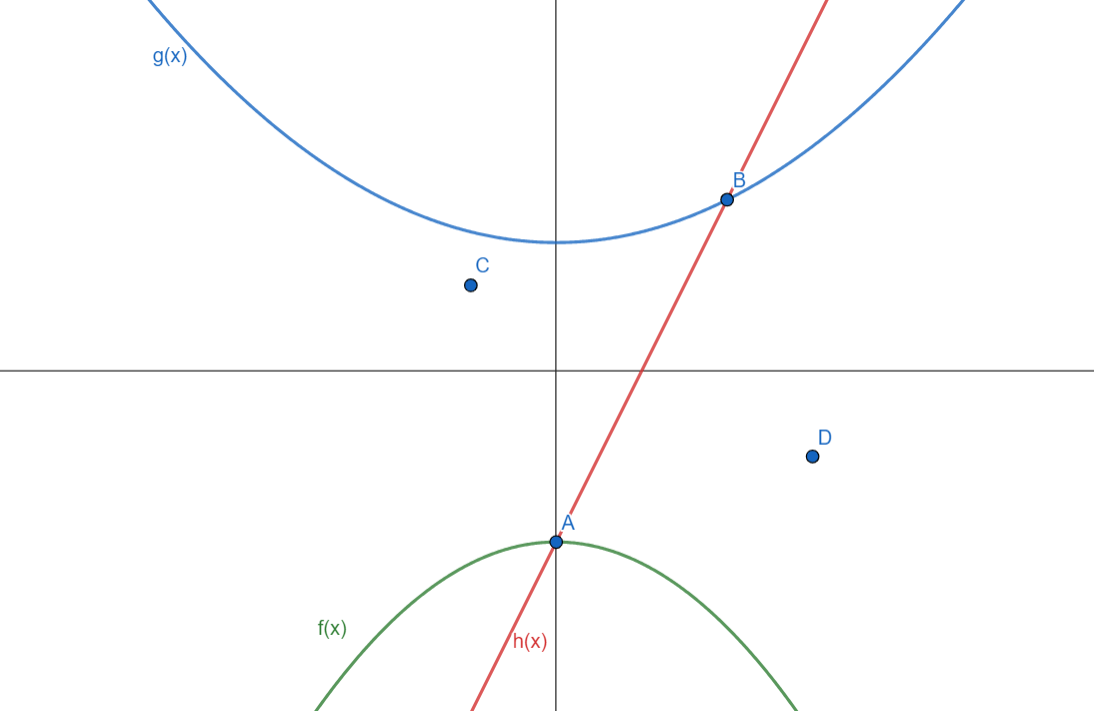
\includegraphics[width=0.6\columnwidth]{figures/zad13.png}
    \label{fig:enter-label}
\end{figure}

\begin{enumerate}
    \item Wyznacz współrzędne punktów $C$ i $D$. (odp. $C=(-1,1), D=(3,-1)$
    \item Wyznacz promień okręgu wpisanego w czworokąt $ABCD$. (odp. $r=\frac{\sqrt{10}}{2}$)

\end{enumerate}